\subsection{Núcleo Magellan: Ferramentas TIC}

\begin{figure}[!htbp]
\centering
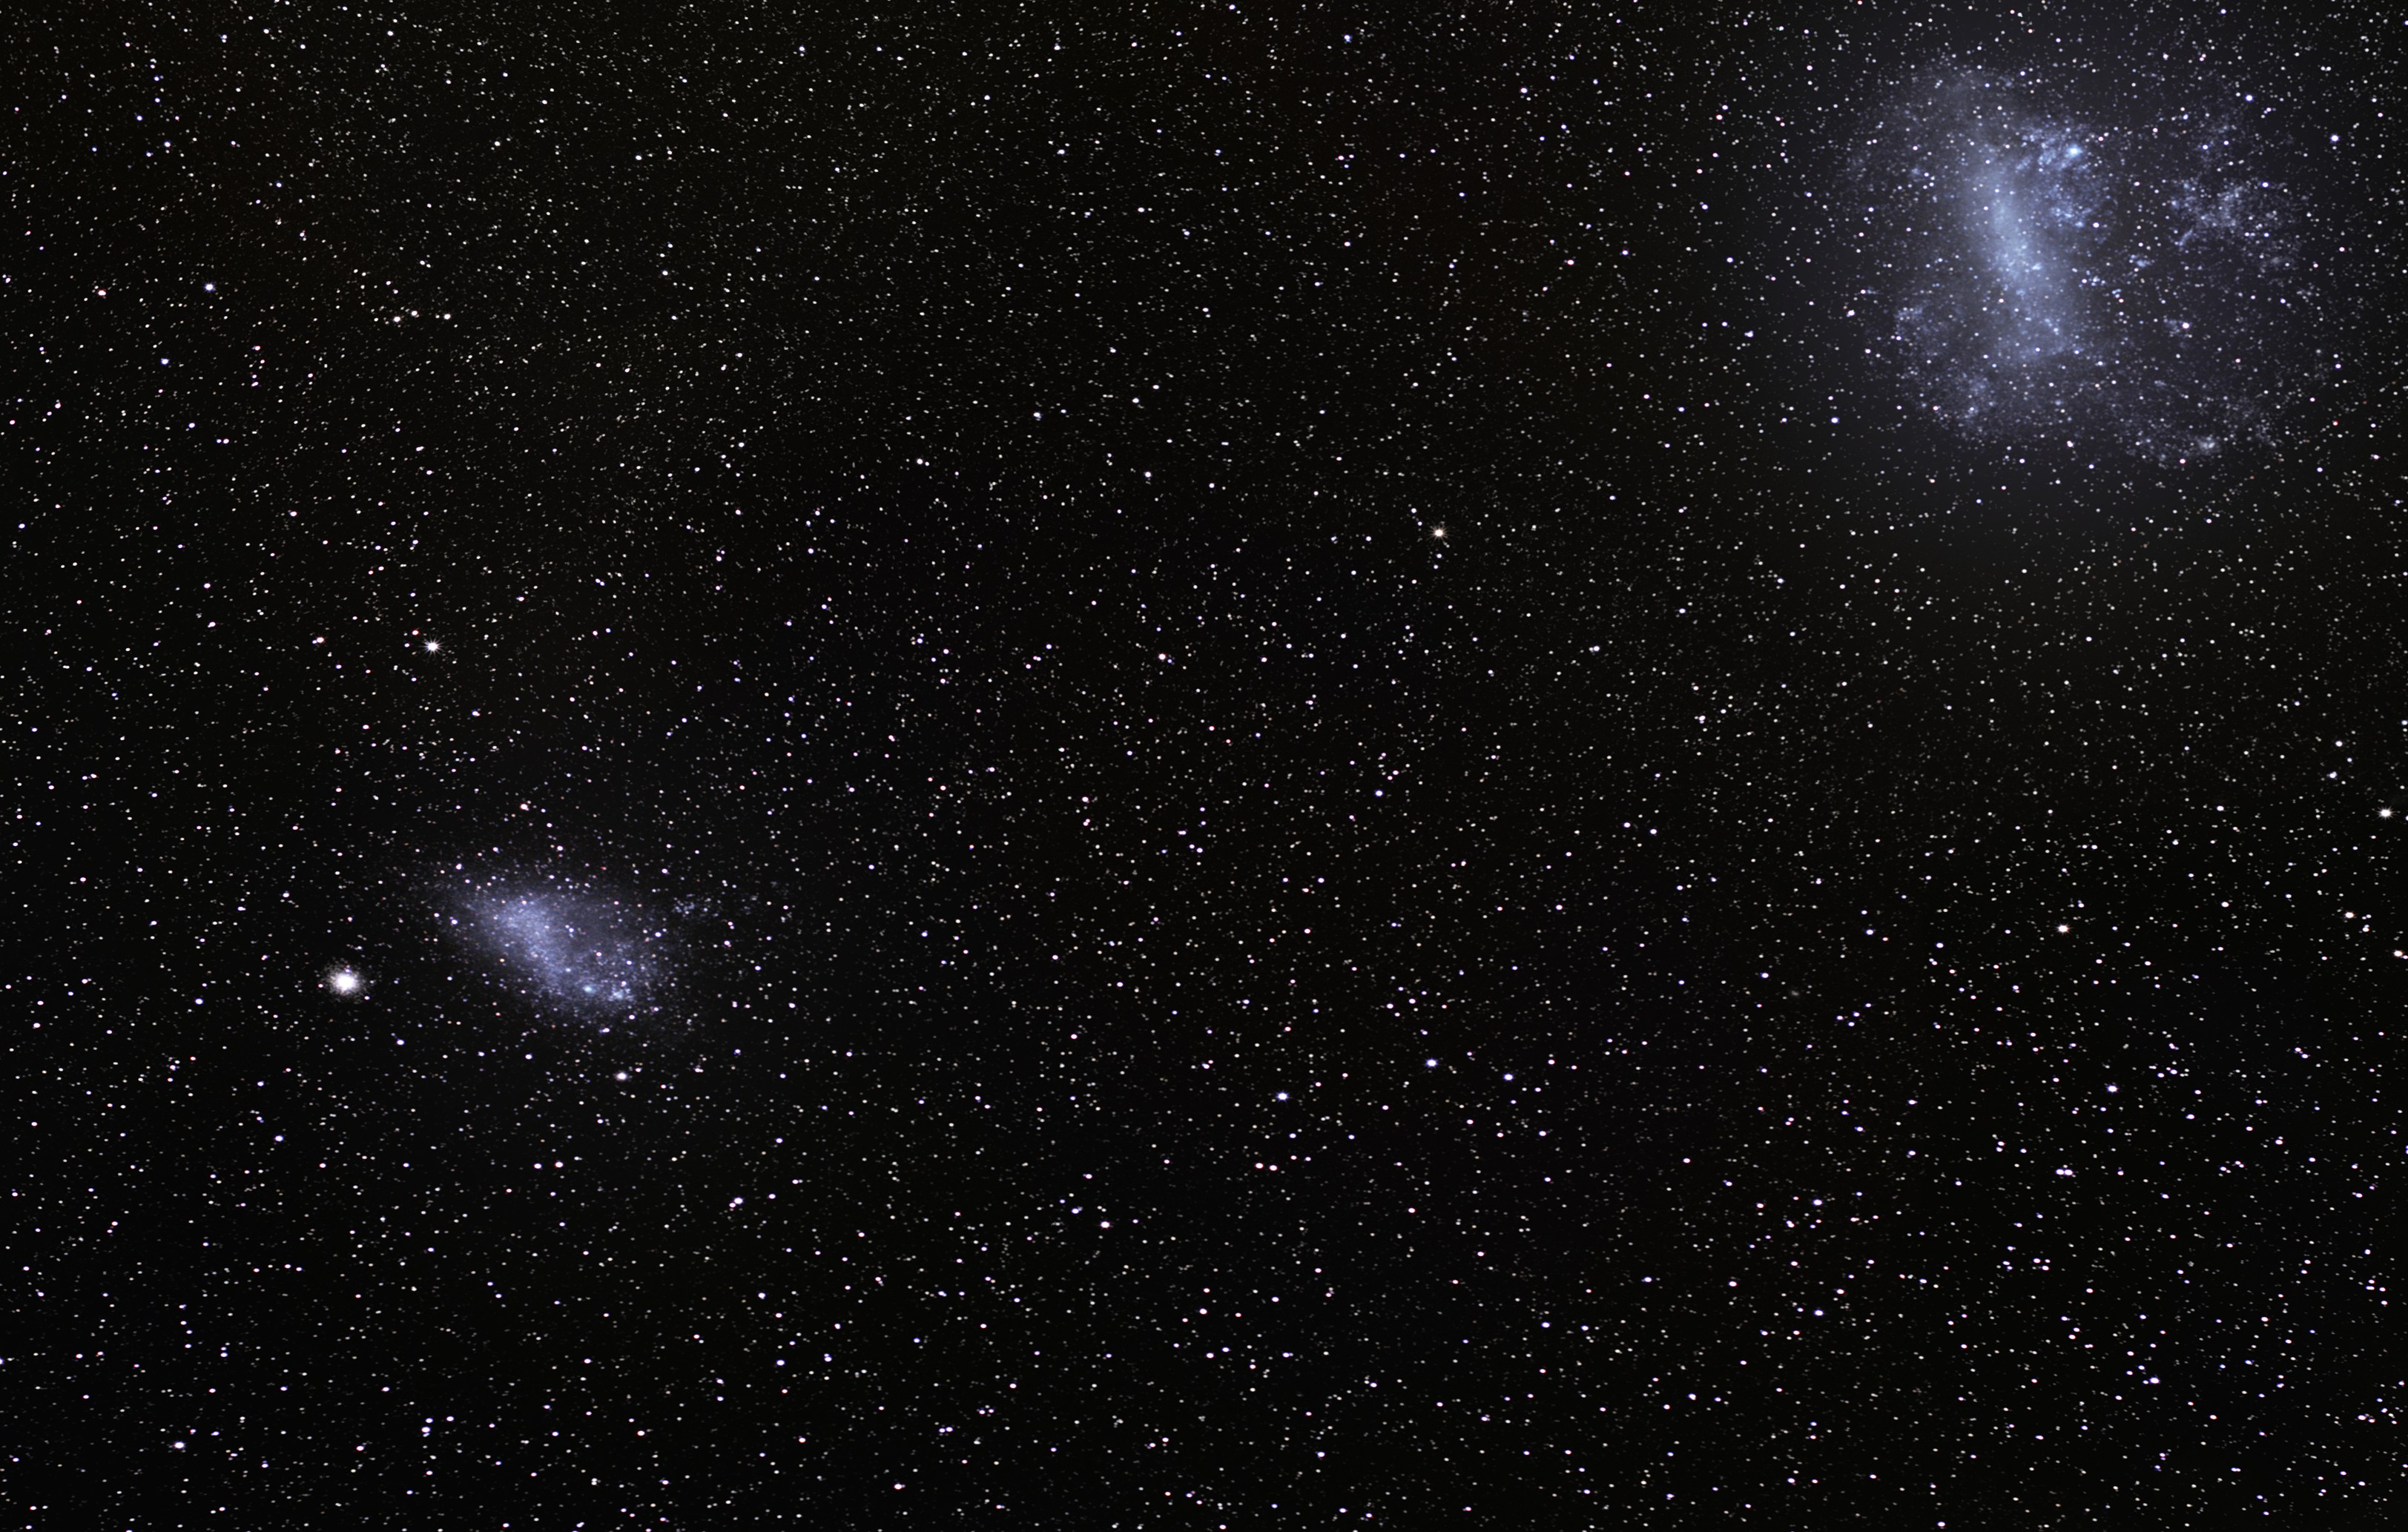
\includegraphics[width=1\linewidth]{files/magellan-d12d937615ed23573ffa3452b507cd3b.jpg}
\end{figure}

\subsubsection{Visão Geral}

O \textbf{Núcleo Magellan} é responsável pelo desenvolvimento e manutenção das ferramentas tecnológicas de informação e comunicação do Projeto Hermathena. Seu nome evoca as nuvens de Magalhães, símbolo de navegação e orientação, representando nossa missão de criar soluções digitais que guiem e potencializem todo o projeto.

\textbf{Afinidade de Área:} Ciência da Computação / Análise e Desenvolvimento de Sistemas / Engenharia de Software

\subsubsection{Missão}

Desenvolver, implementar e manter soluções tecnológicas que automatizem processos, facilitem a gestão de conteúdos e proporcionem experiências digitais inovadoras para os diferentes públicos do BINGO.

\subsubsection{Objetivos Específicos}

\paragraph{1. Desenvolvimento de Sistemas}

\subparagraph{1.1 Portal Web BINGO}

\begin{itemize}
\item[$\square$] Desenvolvimento do site institucional integrado
\item[$\square$] Sistema de gestão de conteúdo (CMS) customizado
\item[$\square$] Área administrativa para equipe
\item[$\square$] Integração com redes sociais
\item[$\square$] Otimização para SEO e acessibilidade
\end{itemize}

\subparagraph{1.2 Sistemas de Automação}

\begin{itemize}
\item[$\square$] Automação de publicações em redes sociais
\item[$\square$] Sistema de agendamento e calendário editorial
\item[$\square$] Automação de relatórios e métricas
\item[$\square$] Chatbot para atendimento e FAQ
\item[$\square$] Integração com APIs de plataformas
\end{itemize}

\subparagraph{1.3 Ferramentas Internas}

\begin{itemize}
\item[$\square$] Sistema de gestão de documentos
\item[$\square$] Dashboard de acompanhamento de indicadores
\item[$\square$] Ferramenta de versionamento colaborativo
\item[$\square$] Sistema de tickets e demandas
\item[$\square$] Wiki interna do projeto
\end{itemize}

\paragraph{2. Infraestrutura Digital}

\subparagraph{2.1 Servidores e Hospedagem}

\bigskip\noindent
\begin{tabular}{p{\dimexpr 0.333\linewidth-2\tabcolsep}p{\dimexpr 0.333\linewidth-2\tabcolsep}p{\dimexpr 0.333\linewidth-2\tabcolsep}}
\toprule
Componente & Especificação & Custo Estimado \\
\hline
\textbf{Servidor NAS} & Synology DS1821+ ou similar, 5x HDD 4TB & R\$ 20.000,00 \\
\textbf{Hospedagem Cloud} & VPS 4vCPU, 8GB RAM, 200GB SSD & R\$ 300,00/mês \\
\textbf{Backup em Nuvem} & 50TB storage + backup automático & R\$ 500,00/mês \\
\bottomrule
\end{tabular}

\bigskip

\subparagraph{2.2 Serviços de IA}

\bigskip\noindent
\begin{tabular}{p{\dimexpr 0.333\linewidth-2\tabcolsep}p{\dimexpr 0.333\linewidth-2\tabcolsep}p{\dimexpr 0.333\linewidth-2\tabcolsep}}
\toprule
Serviço & Uso & Custo Estimado \\
\hline
\textbf{API de IA Generativa} & Chat, assistentes, sumarização & R\$ 200,00/mês \\
\textbf{Geração de Imagens} & Midjourney/DALL-E para materiais & R\$ 50,00/mês \\
\textbf{Análise de Dados} & Processamento de métricas & R\$ 100,00/mês \\
\bottomrule
\end{tabular}

\bigskip

\subparagraph{2.3 Sistema MAM/DAM/VAM}

Sistema integrado de gestão de mídia:

\begin{itemize}
\item \textbf{MAM} (Media Asset Management): Organização de vídeos
\item \textbf{DAM} (Digital Asset Management): Gestão de imagens e documentos
\item \textbf{VAM} (Video Asset Management): Catalogação e versionamento de vídeos
\end{itemize}

\paragraph{3. Automação e Scripts}

\subparagraph{3.1 Automação de Marketing Digital}

\begin{verbatim}
# Exemplo: Pipeline de automação
class ContentAutomation:
    def agendar_conteudo(self, post, data, plataformas):
        """Agenda post em múltiplas plataformas"""
        pass
    
    def gerar_relatorio_metricas(self, periodo):
        """Gera relatório automático de desempenho"""
        pass
    
    def monitorar_mencoes(self):
        """Monitora menções ao BINGO nas redes"""
        pass
\end{verbatim}

\subparagraph{3.2 Web Scraping e Clipping}

\begin{itemize}
\item Monitoramento de notícias sobre BINGO
\item Coleta automática de menções em mídia
\item Análise de sentimento sobre o projeto
\item Alertas de publicações relevantes
\end{itemize}

\subparagraph{3.3 CI/CD e DevOps}

\begin{itemize}
\item Pipeline de deploy automatizado
\item Testes automatizados
\item Monitoramento de uptime
\item Alertas de falhas
\end{itemize}

\paragraph{4. UI/UX e Design de Interação}

\subparagraph{4.1 Design System}

Criação de sistema de design consistente:

\begin{itemize}
\item Biblioteca de componentes reutilizáveis
\item Guia de estilos digital
\item Templates responsivos
\item Protótipos interativos
\end{itemize}

\subparagraph{4.2 Experiência do Usuário}

\begin{itemize}
\item Pesquisa com usuários do portal
\item Testes de usabilidade
\item Análise de heatmaps
\item Otimização de conversão
\end{itemize}

\paragraph{5. Equipamentos de Desenvolvimento}

\bigskip\noindent
\begin{tabular}{p{\dimexpr 0.250\linewidth-2\tabcolsep}p{\dimexpr 0.250\linewidth-2\tabcolsep}p{\dimexpr 0.250\linewidth-2\tabcolsep}p{\dimexpr 0.250\linewidth-2\tabcolsep}}
\toprule
Equipamento & Quantidade & Custo Unitário & Total \\
\hline
\textbf{Monitores 27"} & 3 & R\$ 2.000,00 & R\$ 6.000,00 \\
\textbf{Dispositivos teste (tablets, smartphones)} & 4 & R\$ 2.000,00 & R\$ 8.000,00 \\
\bottomrule
\end{tabular}

\bigskip

\paragraph{6. Software e Assinaturas}

\bigskip\noindent
\begin{tabular}{p{\dimexpr 0.333\linewidth-2\tabcolsep}p{\dimexpr 0.333\linewidth-2\tabcolsep}p{\dimexpr 0.333\linewidth-2\tabcolsep}}
\toprule
Software/Uso & Custo Mensal & Custo Anual \\
\hline
\textbf{Adobe Creative Cloud} (design) & R\$ 200,00 & R\$ 2.400,00 \\
\textbf{Figma Pro} (prototipagem) & R\$ 50,00 & R\$ 600,00 \\
\textbf{Serviços cloud} (AWS/GCP) & R\$ 1.200,00 & R\$ 14.400,00 \\
\bottomrule
\end{tabular}

\bigskip

\subsubsection{Metodologia de Trabalho}

\paragraph{Ciclo de Desenvolvimento}

\paragraph{Stack Tecnológico}

\bigskip\noindent
\begin{tabular}{p{\dimexpr 0.500\linewidth-2\tabcolsep}p{\dimexpr 0.500\linewidth-2\tabcolsep}}
\toprule
Categoria & Tecnologia \\
\hline
\textbf{Frontend} & React / Next.js / Tailwind CSS \\
\textbf{Backend} & Python (Django/FastAPI) / Node.js \\
\textbf{Banco de Dados} & PostgreSQL / Redis \\
\textbf{Mobile} & React Native / Flutter \\
\textbf{DevOps} & Docker / Kubernetes / GitHub Actions \\
\textbf{Cloud} & AWS / Google Cloud Platform \\
\bottomrule
\end{tabular}

\bigskip

\subsubsection{Integração com Outros Núcleos}

\paragraph{Fluxo de Trabalho Integrado}

\subsubsection{Produtos Esperados}

\paragraph{Ano 1}

\bigskip\noindent
\begin{tabular}{p{\dimexpr 0.333\linewidth-2\tabcolsep}p{\dimexpr 0.333\linewidth-2\tabcolsep}p{\dimexpr 0.333\linewidth-2\tabcolsep}}
\toprule
Produto & Descrição & Público \\
\hline
\textbf{Portal Web v1.0} & Site completo com CMS & Geral \\
\textbf{Sistema de Automação} & Agendamento e métricas & Equipe \\
\textbf{Dashboard de Indicadores} & Visualização de KPIs & Gestão \\
\textbf{Chatbot BINGO} & Atendimento automatizado & Visitantes \\
\textbf{App mobile (MVP)} & Versão mobile do portal & Geral \\
\textbf{API pública} & Dados abertos do projeto & Desenvolvedores \\
\bottomrule
\end{tabular}

\bigskip

\subsubsection{Equipe Necessária}

\bigskip\noindent
\begin{tabular}{p{\dimexpr 0.333\linewidth-2\tabcolsep}p{\dimexpr 0.333\linewidth-2\tabcolsep}p{\dimexpr 0.333\linewidth-2\tabcolsep}}
\toprule
Função & Quantidade & Perfil \\
\hline
Coordenador de Núcleo & 1 & Ciência da Computação (Docente) \\
Desenvolvedor Full-stack & 2 & React + Python/Node \\
DevOps / SysAdmin & 1 & Cloud, Docker, CI/CD \\
UX/UI Designer & 1 & Design de interfaces \\
Bolsistas PROBEX & 3 & Ciência da Computação / ADS \\
Voluntários & 5 & Áreas afins \\
\bottomrule
\end{tabular}

\bigskip

\subsubsection{Orçamento Estimado (Ano 1)}

\paragraph{Capital (Material Permanente)}

\bigskip\noindent
\begin{tabular}{p{\dimexpr 0.500\linewidth-2\tabcolsep}p{\dimexpr 0.500\linewidth-2\tabcolsep}}
\toprule
Item & Valor (R\$) \\
\hline
Servidor NAS & 20.000,00 \\
\textbf{Subtotal Capital} & \textbf{81.400,00} \\
\bottomrule
\end{tabular}

\bigskip

\paragraph{Custeio (Mensal/Anual)}

\bigskip\noindent
\begin{tabular}{p{\dimexpr 0.333\linewidth-2\tabcolsep}p{\dimexpr 0.333\linewidth-2\tabcolsep}p{\dimexpr 0.333\linewidth-2\tabcolsep}}
\toprule
Item & Mensal & Anual \\
\hline
Hospedagem cloud & R\$ 150,00 & R\$ 1.800,00 \\
Serviços de IA & R\$ 100,00 & R\$ 1.200,00 \\
Software e licenças & R\$ 180,00 & R\$ 2.160,00 \\
Bolsa (1 bolsista) & R\$ 400,00 & R\$ 2.400,00* \\
\textbf{Subtotal Custeio} & \textbf{R\$ 830,00} & \textbf{R\$ 7.560,00} \\
\bottomrule
\end{tabular}

\bigskip

*6 meses de bolsa

\paragraph{Total Ano 1}

\bigskip\noindent
\begin{tabular}{p{\dimexpr 0.500\linewidth-2\tabcolsep}p{\dimexpr 0.500\linewidth-2\tabcolsep}}
\toprule
Categoria & Valor (R\$) \\
\hline
Capital & 34.000,00 \\
Custeio & 7.560,00 \\
\textbf{TOTAL} & \textbf{41.560,00} \\
\bottomrule
\end{tabular}

\bigskip


\bigskip
\centerline{\rule{13cm}{0.4pt}}
\bigskip

\textit{Documento sujeito a ajustes conforme evolução tecnológica.}